\section{Bibliometric Analysis}
\label{sec:bibliometric}

Before turning to individual methods, this section maps the QIEA
literature as a whole: how large it is, how it has grown over the last
30 years, how much of it is multi-objective, which themes it clusters
into, and which papers have been most influential. It complements the
targeted selection of Section~\ref{sec:introduction:scope}: that
selection decides which methods the taxonomy examines in depth, while
this section gives the field-level context in which to read them.

\subsection{Data and Method}
\label{sec:bibliometric:method}

We queried OpenAlex~\citep{priem2022openalex}, a fully open index of
scholarly works covering all major publishers, on 3 October 2026. Two
queries were run against titles and abstracts, restricted to
publication years 1996--2026:
\begin{itemize}
  \item \textbf{QIEA query:} \texttt{"quantum-inspired evolutionary" OR
    "quantum-inspired genetic" OR "quantum evolutionary algorithm" OR
    "quantum genetic algorithm" OR QIEA}. This is the corpus analysed in
    the rest of this section.
  \item \textbf{Broad query:} \texttt{("evolutionary computation" OR
    "evolutionary algorithm" OR "genetic algorithm") AND ("quantum
    computing" OR "quantum computer")}. This captures the wider
    intersection of evolutionary computation and quantum computing,
    including the second research thread of
    Section~\ref{sec:introduction} (evolutionary algorithms applied
    \emph{to} quantum problems), and is used only for the publication
    trend.
\end{itemize}
Each result set was then cleaned in four steps. (1) Only peer-reviewed
document types were kept (journal articles, conference papers, book
chapters, books, reviews, and dissertations), dropping preprints,
software, and datasets; this removed, among others, several dozen
near-duplicate repository uploads dated 2026. (2) Only English-language
records were kept, matching Section~\ref{sec:introduction:scope}. (3)
Each record's title and abstract, as returned by OpenAlex, was checked
locally for the query terms. OpenAlex also matches records on text it
does not return, such as some publisher-withheld abstracts, and this
step removed off-topic matches (e.g.\ quantum-dot physics papers) at the
cost of also dropping some genuine records whose abstract is not
available. (4) Records with the same normalized title were merged,
keeping the most-cited version. The QIEA query went from 2{,}835
records to 2{,}654, 2{,}603, 2{,}341, and finally 2{,}250 papers; the
broad query from 935 to 558. Two publication years were corrected by
hand where OpenAlex disagreed with the paper's own DOI
(\citet{narayanan1996qiga}, dated 2002 in OpenAlex, and
\citet{han2001pqga}, also dated 2002).

A paper was tagged multi-objective if its title, abstract, or keywords
mention multi-, many-, bi-, two-, three-, or four-objective
optimization or Pareto optimality. Keyword clusters were built from
the keywords OpenAlex assigns to each paper: synonyms were merged, the
query terms themselves (present in nearly every record) were removed,
and keywords occurring in at least 20 papers were kept. This gave 55
keywords, linked whenever two of them occur in the same paper and
weighted by the number of such papers (695 links). Clusters were
found with the Louvain method~\citep{blondel2008louvain}. Citation
counts are as reported by OpenAlex on the retrieval date. The full
pipeline (queries, cleaning, figures, and tables) is a single script,
\texttt{bibliometric\_analysis.py}, distributed with the paper together
with the raw query results it was run on, so every number in this
section can be regenerated.

\subsection{Publication Trend}
\label{sec:bibliometric:trend}

Figure~\ref{fig:bibliometric-trend}(a) shows the QIEA corpus by year.
After \citet{narayanan1996qiga}'s 1996 paper, the field is almost empty
until Han and Kim's papers of 2001--2004~\citep{han2001pqga,han2002qea,han2004hepsilon},
then grows quickly, from 24 papers in 2004 to a peak of 166 in 2010
and a second peak of 164 in 2013. Output then falls to 74 papers in
2017 before recovering to 135 in 2025; with 130 papers by early October,
2026 is on course to exceed it.

Multi-objective work is a small but growing part of this corpus: 215 of
the 2{,}250 papers (9.6\%) are tagged multi-objective. The share was
7.6\% up to 2013 and 8.7\% over 2014--2023, then roughly doubled to
16.6\% over 2024--2026 (61 of 367 papers). The recent recovery of the
field as a whole is therefore disproportionately multi-objective, which
is part of the case for a survey focused on QIEA-for-MOO specifically.

The broad query (Figure~\ref{fig:bibliometric-trend}(b)) follows a
different curve: between 7 and 24 papers a year over 2005--2020, then a
sharp rise from 2021, reaching 63 papers in 2024 and 99 in 2025. The 2026
figure (40 papers) is partial and should not be read as a decline. The
composition of this corpus changes with its growth. Over 2005--2020,
138 of its 241 papers (57\%) also belong to the QIEA corpus, and only 24
(10\%) mention quantum circuits, variational algorithms, QAOA, or
similar quantum problems in their title or abstract. Over 2021--2026,
only 97 of 294 (33\%) are QIEA papers, while 87 (30\%) mention such
quantum problems. The recent growth at the intersection of evolutionary
computation and quantum computing therefore comes mostly from
evolutionary algorithms applied \emph{to} quantum problems, the thread
this survey's case study belongs to, rather than from quantum-inspired
algorithms, and coincides with the availability of the NISQ hardware
discussed in Section~\ref{sec:introduction}.

\begin{figure}[htbp]
  \centering
  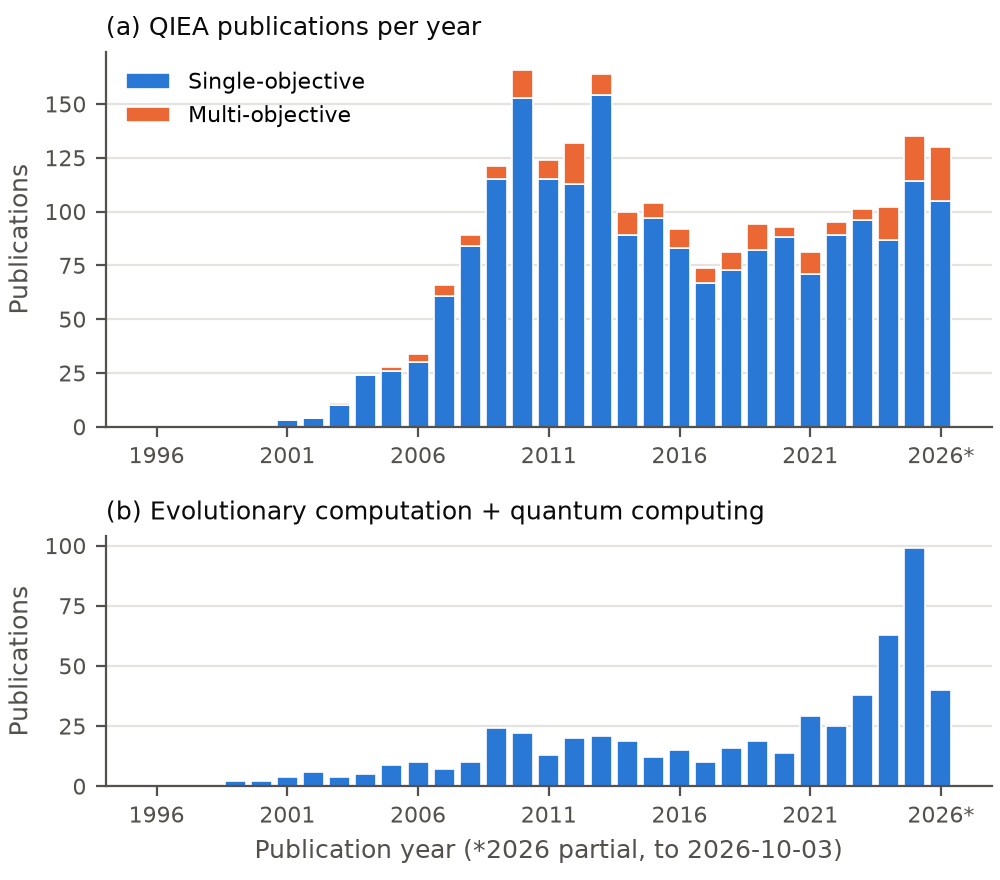
\includegraphics[width=\linewidth]{figures/bibliometric_trend.png}
  \caption{Publications per year, 1996--2026, from OpenAlex after
    cleaning (Section~\ref{sec:bibliometric:method}). (a) QIEA query
    (2{,}250 papers), split into single-objective and multi-objective
    papers. (b) Broad query on evolutionary computation and quantum
    computing (558 papers). 2026 covers papers indexed up to 3 October
    2026 only.}
  \label{fig:bibliometric-trend}
\end{figure}

\subsection{Keyword Clusters}
\label{sec:bibliometric:clusters}

The keyword network splits into four clusters
(Figure~\ref{fig:bibliometric-clusters},
Table~\ref{tab:bibliometric-clusters}):
\begin{description}
  \item[Cluster 1, search dynamics and operators (20 keywords).]
    Convergence rate, premature convergence, the quantum rotation gate,
    population diversity, and the exploration--exploitation balance.
    This is the algorithm-design core of the field, corresponding to
    the representation and operator axes of
    Sections~\ref{sec:taxonomy:representation}
    and~\ref{sec:taxonomy:operator}.
  \item[Cluster 2, combinatorial benchmarks (9 keywords).]
    Combinatorial optimization, the knapsack and travelling salesman
    problems, and superposition: the lineage of the original
    single-objective papers~\citep{narayanan1996qiga,han2002qea}.
  \item[Cluster 3, multi-objective engineering applications (15
    keywords).] Multi-objective optimization and the Pareto front,
    together with wireless sensor networks, power-loss reduction,
    distributed generation, makespan minimization, resource allocation,
    and energy efficiency.
  \item[Cluster 4, hybrids with other methods (11 keywords).] Genetic
    algorithms, particle swarm optimization (including its
    quantum-behaved variant), feature selection, support vector
    machines, and hyperparameter optimization: QIEAs combined with, or
    compared against, other metaheuristics and machine-learning models.
\end{description}
The most informative feature of this structure for this survey is
where multi-objective optimization sits. It does not cluster with the
operator and convergence vocabulary of Cluster 1, but with application
domains. In other words, the multi-objective QIEA literature is
organized mainly around \emph{what} is being optimized, not around how
a quantum-inspired operator should change when there are several
objectives. This is consistent with the hybridization pattern found in
Section~\ref{sec:taxonomy:hybridization} (a QIEA operator grafted onto
an unchanged classical MOEA) and with the under-specified reference
solution discussed in Section~\ref{sec:critical-analysis:so-to-mo}.
The keywords are assigned automatically by OpenAlex rather than by the
authors, so this reading should be taken as indicative rather than
definitive.

\begin{figure}[htbp]
  \centering
  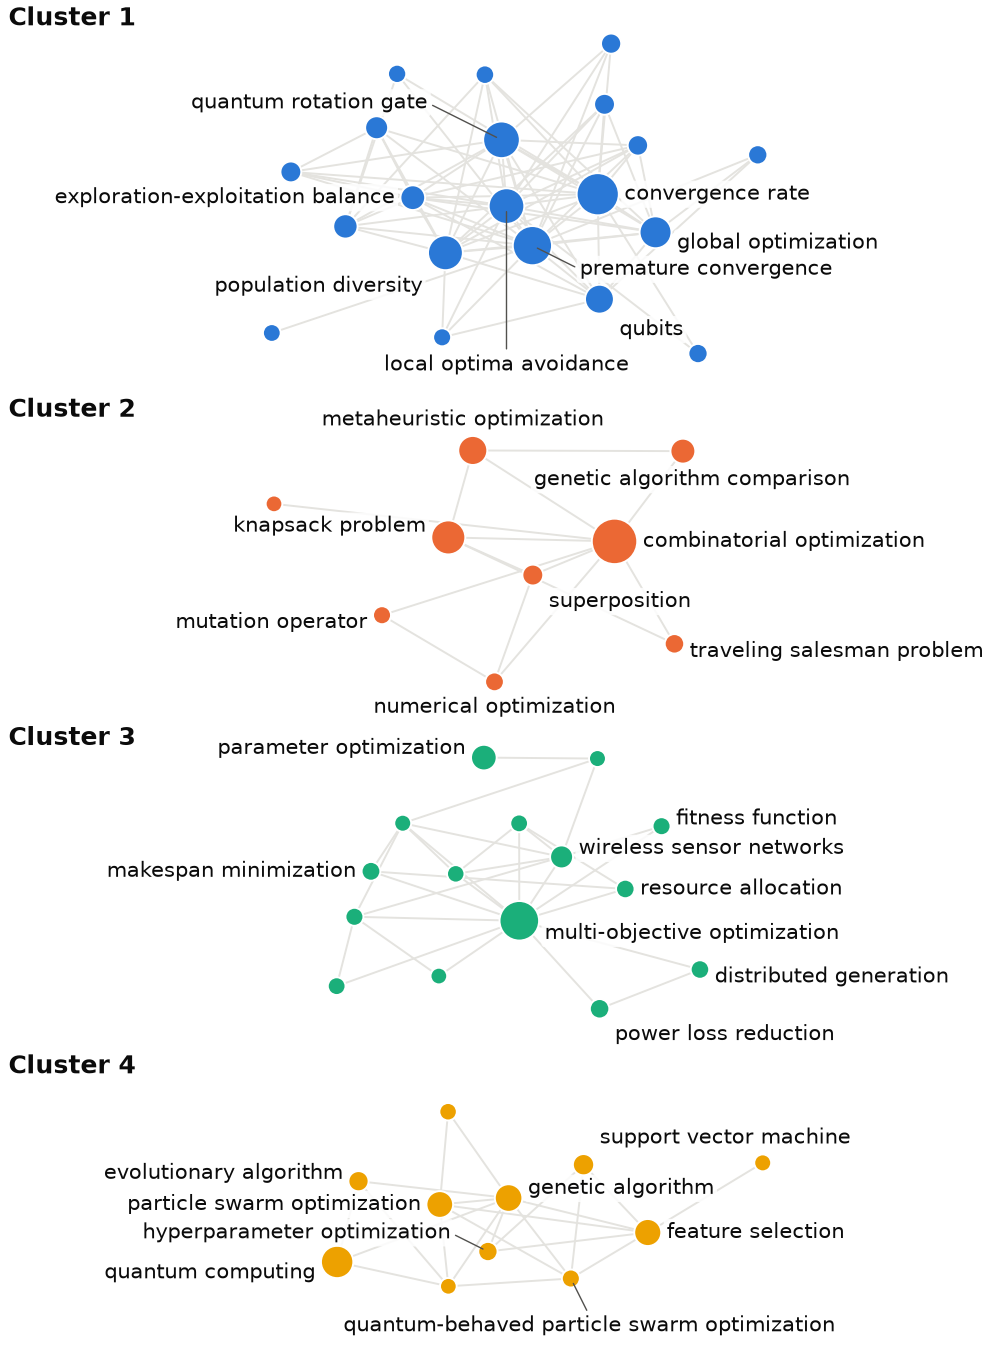
\includegraphics[width=\linewidth]{figures/bibliometric_clusters.png}
  \caption{Keyword co-occurrence clusters in the QIEA corpus (55
    keywords occurring in at least 20 papers; Louvain clustering).
    Node size is proportional to the number of papers with that
    keyword; within each cluster, the stronger half of co-occurrence
    links is drawn and the eight most frequent keywords are labelled.
    Links between clusters are not drawn. The full keyword list per
    cluster is in Table~\ref{tab:bibliometric-clusters}.}
  \label{fig:bibliometric-clusters}
\end{figure}

\begin{table}[htbp]
  \centering
  \small
  \caption{Keywords in each cluster of
    Figure~\ref{fig:bibliometric-clusters}, most frequent first.}
  \label{tab:bibliometric-clusters}
  \begin{tabularx}{\linewidth}{@{}p{3.2cm}X@{}}
    \toprule
    Cluster & Keywords \\
    \midrule
    1. Search dynamics and operators &
      convergence rate, premature convergence, quantum rotation gate,
      local optima avoidance, population diversity, global optimization,
      qubits, exploration-exploitation balance, hybrid metaheuristic,
      local search, function optimization, global search, continuous
      optimization, global search ability, BP neural network,
      real-coded genetic algorithm, benchmark functions, simulated
      annealing, image segmentation, NP-hard combinatorial optimization \\
    2. Combinatorial benchmarks &
      combinatorial optimization, knapsack problem, metaheuristic
      optimization, genetic algorithm comparison, superposition,
      traveling salesman problem, numerical optimization, mutation
      operator, NP-complete problems \\
    3. Multi-objective engineering applications &
      multi-objective optimization, parameter optimization, wireless
      sensor networks, power loss reduction, makespan minimization,
      distributed generation, resource allocation, fitness function,
      Pareto front, energy efficiency, Pareto optimal solutions, quality
      of service, clustering, energy consumption, solution diversity \\
    4. Hybrids with other methods &
      quantum computing, genetic algorithm, feature selection, particle
      swarm optimization, support vector machine, evolutionary
      algorithm, hyperparameter optimization, quantum-behaved particle
      swarm optimization, parameter estimation, dimensionality
      reduction, quantum-inspired algorithms \\
    \bottomrule
  \end{tabularx}
\end{table}

\subsection{Most-Cited Papers}
\label{sec:bibliometric:top-cited}

Table~\ref{tab:bibliometric-top-cited} lists the ten most-cited papers
in the QIEA corpus. Three patterns stand out. First, the list is old:
apart from \citet{narayanan1996qiga}, eight of the ten papers date from
2001--2010 and only one from the last decade, which partly reflects
the time citations take to accumulate. Second, it is dominated by one research group: Han, Kim,
and colleagues authored three of the ten, including the top-ranked
paper, which alone has more than twice the citations of any other.
Third, only two of the ten are multi-objective~\citep{li2007hqga,deng2020gate},
and both are application papers that hybridize a QIEA with another
method, not papers about multi-objective QIEA design as such. The
single-objective papers are the ones the field's representation and
operators were built from, which is why
Section~\ref{sec:taxonomy:objectives} uses them as the baseline for the
multi-objective methods. Each paper is summarized briefly below, in rank
order.

\begin{table}[htbp]
  \centering
  \small
  \caption{The ten most-cited papers in the QIEA corpus (OpenAlex
    citation counts, 3 October 2026). Year is the year OpenAlex
    records, which for journal papers can be the year of online
    publication rather than of the printed volume.}
  \label{tab:bibliometric-top-cited}
  \begin{tabularx}{\linewidth}{@{}rlXrr@{}}
    \toprule
    \# & Paper & Contribution & Year & Citations \\
    \midrule
    1 & \citet{han2002qea} & QEA: Q-bit chromosome and Q-gate & 2002 & 1{,}589 \\
    2 & \citet{narayanan1996qiga} & First quantum-inspired GA & 1996 & 648 \\
    3 & \citet{han2004hepsilon} & H$_\epsilon$ gate, termination criterion & 2004 & 482 \\
    4 & \citet{deng2020gate} & Multi-objective airport gate allocation & 2020 & 339 \\
    5 & \citet{zhang2011qieasurvey} & QIEA survey and empirical study & 2010 & 297 \\
    6 & \citet{li2007hqga} & Multi-objective flow-shop scheduling & 2007 & 208 \\
    7 & \citet{zhao2009cognitive} & Cognitive-radio spectrum allocation & 2009 & 205 \\
    8 & \citet{lee2011qgadispatch} & Economic dispatch with wind power & 2010 & 194 \\
    9 & \citet{han2001pqga} & Parallel QGA & 2001 & 191 \\
    10 & \citet{platel2009qeaeda} & QEA as an estimation-of-distribution algorithm & 2008 & 175 \\
    \bottomrule
  \end{tabularx}
\end{table}

\textbf{1. \citet{han2002qea}.} Introduces the quantum-inspired
evolutionary algorithm (QEA): individuals are strings of Q-bits, each a
probabilistic superposition of 0 and 1, and a Q-gate (rotation gate)
drives them toward better solutions. On the knapsack problem, QEA
performs well even with a small population and without the premature
convergence of a conventional genetic algorithm. This is the
representation and operator described in
Section~\ref{sec:background:quantum}, and the one nearly every later
method in this survey builds on.

\textbf{2. \citet{narayanan1996qiga}.} The first quantum-inspired
genetic algorithm. Drawing on the many-universes interpretation of
quantum mechanics, it runs several populations (``universes'') in
parallel and combines them with an interference crossover, compared
against a classical genetic algorithm on the travelling salesman
problem. The quantum-inspired version is shown, informally, to perform
better on a small instance. It predates the Q-bit chromosome, and is
the only method in this survey built around interference
(Section~\ref{sec:taxonomy:operator}).

\textbf{3. \citet{han2004hepsilon}.} Improves QEA in three ways: a
termination criterion that gives a clearer meaning to the convergence
of Q-bit individuals, the H$_\epsilon$ gate (a rotation gate that keeps
each Q-bit probability away from exactly 0 or 1), and a two-phase
scheme that tunes the Q-bits' initial conditions in a first phase.
Tested on numerical and combinatorial problems, the updated QEA
improves convergence speed, fitness, and robustness over the original.

\textbf{4. \citet{deng2020gate}.} A three-objective airport gate
allocation model (passenger walking distance, balance of idle time
across gates, and use of large gates), solved by IPOQEA, a QEA
combined with a niche co-evolution strategy and an enhanced particle
swarm optimizer. Validated on operational data from Baiyun Airport. The only paper of the last decade in the list, and one of its
two multi-objective papers; the abstract does not state whether the
three objectives are handled by Pareto ranking or combined into one.

\textbf{5. \citet{zhang2011qieasurvey}.} A survey of QIEAs on
classical computers that proposes a unified framework for them,
reviews their theoretical development and their applications from
combinatorial to numerical optimization, and compares the performance
of different QIEA types empirically. It is the most-cited general
survey of the field.

\textbf{6. \citet{li2007hqga}.} A hybrid quantum-inspired genetic
algorithm for multi-objective flow-shop scheduling. A Q-bit genetic
algorithm explores the binary space, with a random-key decoding that
turns Q-bit strings into job permutations, while a permutation-based
genetic algorithm explores and refines schedules directly. The two
parts handle multiple objectives differently: the Q-bit part uses a
randomly weighted sum of the objectives, while the permutation part
uses non-dominated sorting with two population-trimming techniques for
diversity. The random weighting is one of the few documented answers to the
reference-solution question of Section~\ref{sec:taxonomy:objectives}:
for any one weight vector there is again a single best solution to
rotate toward.

\textbf{7. \citet{zhao2009cognitive}.} Formulates spectrum allocation in
cognitive radio as an optimization problem and solves it with a
genetic algorithm, a quantum genetic algorithm, and particle swarm
optimization, using a mapping between the channel-assignment matrix and
each algorithm's encoding to shrink the search space. All three
outperform the commonly used colour-sensitive graph-colouring
algorithm. The QIEA here is one of three interchangeable optimizers
rather than the paper's focus, an early example of the comparative
application papers that Cluster 4 captures.

\textbf{8. \citet{lee2011qgadispatch}.} Applies a quantum genetic
algorithm to dynamic economic dispatch in a power system with
valve-point effects and wind generation, reporting that it finds the
minimum-cost dispatch quickly and accurately. Its published abstract gives no further detail of
the algorithm; it is representative of the power-system applications
that appear in Cluster 3.

\textbf{9. \citet{han2001pqga}.} A parallel quantum-inspired genetic
algorithm (PQGA). It argues that the Q-bit representation's rapid
convergence and global search make QIEAs well suited to parallel,
multi-population structures, and shows on the knapsack problem that
PQGA outperforms both the sequential QGA and conventional genetic
algorithms.

\textbf{10. \citet{platel2009qeaeda}.} Shows that QEA belongs to the
class of estimation-of-distribution algorithms (EDAs): its Q-bit
population is a set of probabilistic models of promising solutions.
Compared with three classical EDAs, QEA does well on loss of
diversity, scalability, solution quality, and robustness to fitness
noise, which the authors attribute to its multimodel nature: it adapts
its learning speed and can represent more complex distributions than a
single-model EDA. This reframing matters for the multi-objective case,
where a single probabilistic model has to cover a whole Pareto front
rather than one optimum.

\subsection{Limitations of the Analysis}
\label{sec:bibliometric:limitations}

Four limitations apply. OpenAlex has broad coverage but imperfect
metadata: the two publication-year errors corrected above were found
only because they affected highly cited papers, and others may remain
in the long tail. The keywords are assigned automatically, not by
authors, so the clusters describe OpenAlex's reading of each abstract.
The multi-objective tag is a text match, which will miss papers that
describe several objectives without these terms and include some that
mention them only in passing. Citation counts favour older papers and
change over time; the ranking above is a snapshot as of the retrieval
date.
